% Figure 2: Feasible Set + Projection Π_C — Geometric Diagram
% Compile: pdflatex fig2_feasible_set.tex
\documentclass[border=8pt]{standalone}
\usepackage{tikz}
\usepackage{amsmath,amssymb}
\usetikzlibrary{
  arrows.meta,
  calc,
  positioning,
  decorations.pathreplacing,
  decorations.markings,
  patterns,
  fit,
  backgrounds,
  shadows.blur
}

\definecolor{feasblue}{HTML}{2980B9}
\definecolor{feasfill}{HTML}{D6EAF8}
\definecolor{projred}{HTML}{C0392B}
\definecolor{unconstr}{HTML}{E74C3C}
\definecolor{constrgrn}{HTML}{27AE60}
\definecolor{annotgray}{HTML}{7F8C8D}
\definecolor{bgcard}{HTML}{FDFEFE}
\definecolor{violetlog}{HTML}{8E44AD}

\begin{document}
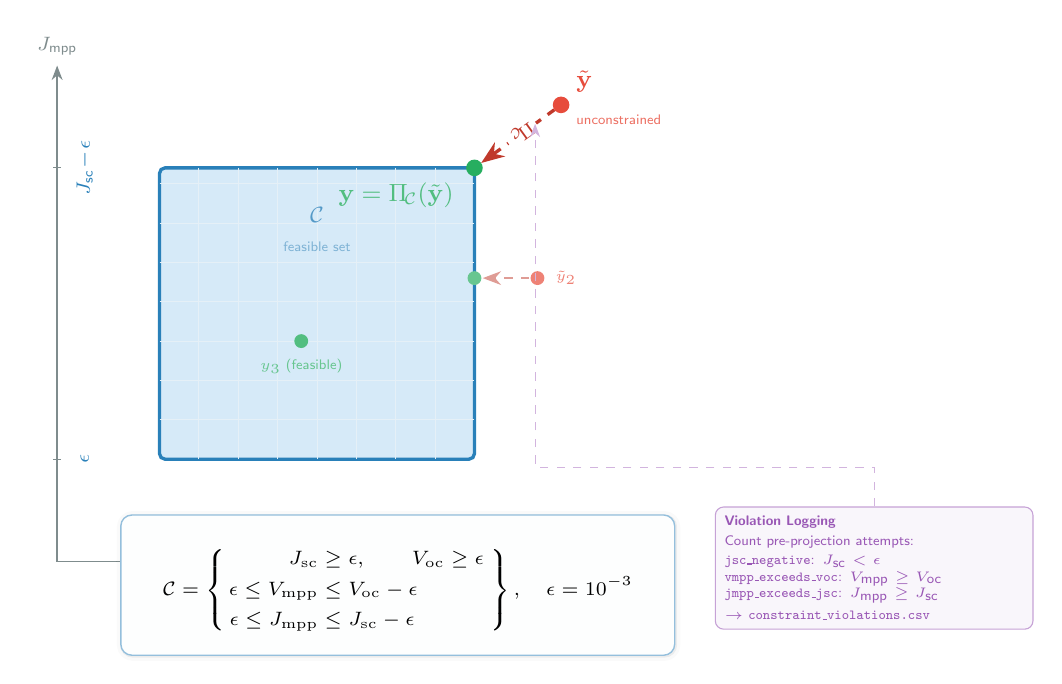
\begin{tikzpicture}[
  >=Stealth,
  every node/.style={font=\sffamily\small},
  annot/.style={font=\sffamily\scriptsize, text=annotgray},
]

% ═══════════════════════════════════════════
% COORDINATE AXES
% ═══════════════════════════════════════════
\draw[->, line width=0.5pt, annotgray] (-0.8, -0.8) -- (6.2, -0.8)
  node[right, font=\sffamily\scriptsize] {$V_{\text{mpp}}$};
\draw[->, line width=0.5pt, annotgray] (-0.8, -0.8) -- (-0.8, 5.5)
  node[above, font=\sffamily\scriptsize] {$J_{\text{mpp}}$};

% Axis labels
\node[annot] at (3.0, -1.15) {(projected onto 2 of 4 dimensions)};

% ═══════════════════════════════════════════
% FEASIBLE REGION C (shaded box)
% ═══════════════════════════════════════════
% The box represents: ε ≤ Vmpp ≤ Voc-ε, ε ≤ Jmpp ≤ Jsc-ε
\coordinate (Cbl) at (0.5, 0.5);  % bottom-left
\coordinate (Ctr) at (4.5, 4.2);  % top-right

% Shaded interior
\fill[feasfill, rounded corners=2pt] (Cbl) rectangle (Ctr);

% Hatched boundary for "active constraint" feel
\draw[feasblue, line width=1.2pt, rounded corners=2pt] (Cbl) rectangle (Ctr);

% Subtle grid inside feasible set
\foreach \x in {1.0, 1.5, ..., 4.0} {
  \draw[feasblue!12, line width=0.3pt] (\x, 0.5) -- (\x, 4.2);
}
\foreach \y in {1.0, 1.5, ..., 4.0} {
  \draw[feasblue!12, line width=0.3pt] (0.5, \y) -- (4.5, \y);
}

% Label feasible set
\node[font=\sffamily\footnotesize, text=feasblue!80] at (2.5, 3.6) {
  $\mathcal{C}$
};
\node[font=\sffamily\tiny, text=feasblue!60] at (2.5, 3.2) {
  feasible set
};

% Boundary labels
\node[annot, text=feasblue] at (0.5, -0.45) {$\epsilon$};
\node[annot, text=feasblue] at (4.5, -0.45) {$V_{\text{oc}}\!-\!\epsilon$};
\node[annot, text=feasblue, rotate=90] at (-0.45, 0.5) {$\epsilon$};
\node[annot, text=feasblue, rotate=90] at (-0.45, 4.2) {$J_{\text{sc}}\!-\!\epsilon$};

% Tick marks on axes
\draw[annotgray, line width=0.4pt] (0.5,-0.85) -- (0.5,-0.75);
\draw[annotgray, line width=0.4pt] (4.5,-0.85) -- (4.5,-0.75);
\draw[annotgray, line width=0.4pt] (-0.85,0.5) -- (-0.75,0.5);
\draw[annotgray, line width=0.4pt] (-0.85,4.2) -- (-0.75,4.2);

% ═══════════════════════════════════════════
% UNCONSTRAINED POINT (outside)
% ═══════════════════════════════════════════
\coordinate (ytilde) at (5.6, 5.0);

\fill[unconstr] (ytilde) circle (3pt);
\node[font=\sffamily\small, text=unconstr, above right=1pt and 2pt of ytilde] {
  $\tilde{\mathbf{y}}$
};
\node[annot, text=unconstr!80, below right=0pt and 2pt of ytilde] {
  \tiny unconstrained
};

% ═══════════════════════════════════════════
% PROJECTED POINT (on boundary)
% ═══════════════════════════════════════════
\coordinate (yproj) at (4.5, 4.2);

\fill[constrgrn] (yproj) circle (3pt);
\node[font=\sffamily\small, text=constrgrn!80, below left=2pt and 4pt of yproj] {
  $\mathbf{y} = \Pi_{\!\mathcal{C}}(\tilde{\mathbf{y}})$
};

% ═══════════════════════════════════════════
% PROJECTION ARROW (red dashed)
% ═══════════════════════════════════════════
\draw[
  ->,
  projred,
  line width=1.2pt,
  dashed,
  shorten >=3pt,
  shorten <=3pt,
  decoration={markings, mark=at position 0.55 with {\arrow[projred,line width=1.2pt]{Stealth}}},
  postaction={decorate}
] (ytilde) -- (yproj);

% Label on arrow
\node[
  font=\sffamily\scriptsize\bfseries,
  text=projred,
  fill=white,
  inner sep=1.5pt,
  rotate={atan2(4.2-5.0, 4.5-5.6)}
] at ($(ytilde)!0.45!(yproj)$) {
  $\Pi_{\!\mathcal{C}}$
};

% ═══════════════════════════════════════════
% SECOND EXAMPLE POINT (less extreme violation)
% ═══════════════════════════════════════════
\coordinate (ytilde2) at (5.3, 2.8);
\coordinate (yproj2) at (4.5, 2.8);

\fill[unconstr!70] (ytilde2) circle (2.5pt);
\node[annot, text=unconstr!70, right=3pt of ytilde2] {\tiny $\tilde{y}_2$};

\fill[constrgrn!70] (yproj2) circle (2.5pt);

\draw[->, projred!50, line width=0.8pt, dashed, shorten >=3pt, shorten <=3pt]
  (ytilde2) -- (yproj2);

% ═══════════════════════════════════════════
% THIRD EXAMPLE (inside — no projection needed)
% ═══════════════════════════════════════════
\coordinate (yinside) at (2.3, 2.0);
\fill[constrgrn!80] (yinside) circle (2.5pt);
\node[annot, text=constrgrn!70, below=3pt of yinside] {\tiny $y_3$ (feasible)};

% ═══════════════════════════════════════════
% CONSTRAINT SET DEFINITION BOX
% ═══════════════════════════════════════════
\node[
  draw=feasblue!50,
  fill=bgcard,
  rounded corners=4pt,
  line width=0.5pt,
  font=\scriptsize,
  text width=6.8cm,
  align=left,
  below=0.7cm of Cbl,
  anchor=north west,
  xshift=-0.5cm,
  blur shadow={shadow blur steps=2, shadow xshift=0.3pt, shadow yshift=-0.3pt, shadow opacity=15}
] (constraintbox) {
  \vspace{-2pt}
  \begin{equation*}
    \mathcal{C} = \left\{\,
    \begin{aligned}
      J_{\text{sc}} &\ge \epsilon, \qquad
      V_{\text{oc}} \ge \epsilon \\
      \epsilon \le V_{\text{mpp}} &\le V_{\text{oc}} - \epsilon \\
      \epsilon \le J_{\text{mpp}} &\le J_{\text{sc}} - \epsilon
    \end{aligned}
    \;\right\}, \quad \epsilon = 10^{-3}
  \end{equation*}
  \vspace{-6pt}
};

% ═══════════════════════════════════════════
% VIOLATION LOGGING CALLOUT
% ═══════════════════════════════════════════
\node[
  draw=violetlog!50,
  fill=violetlog!5,
  rounded corners=3pt,
  line width=0.4pt,
  font=\sffamily\tiny,
  text=violetlog!90,
  text width=3.8cm,
  align=left,
  right=0.5cm of constraintbox.north east,
  anchor=north west,
  yshift=0.1cm
] (logbox) {
  \textbf{Violation Logging}\\[1pt]
  Count pre-projection attempts:\\[1pt]
  \texttt{jsc\_negative}: $J_{\text{sc}} < \epsilon$\\
  \texttt{vmpp\_exceeds\_voc}: $V_{\text{mpp}} \ge V_{\text{oc}}$\\
  \texttt{jmpp\_exceeds\_jsc}: $J_{\text{mpp}} \ge J_{\text{sc}}$\\[2pt]
  $\rightarrow$ \texttt{constraint\_violations.csv}
};

% Arrow from log box to projection
\draw[->, violetlog!40, line width=0.4pt, dashed]
  (logbox.north) -- ++(0, 0.5) -| ($(ytilde)!0.3!(yproj)$);

\end{tikzpicture}
\end{document}
